\documentclass[tikz,border=10pt]{standalone}
\usepackage[T1]{fontenc}
\usepackage{lmodern}
\usetikzlibrary{arrows.meta,calc,fit,backgrounds,positioning}

\definecolor{blueband}{HTML}{DDEEF9}
\definecolor{blueborder}{HTML}{3B82C4}
\definecolor{yellowband}{HTML}{FDECB8}
\definecolor{yellowborder}{HTML}{E08E1D}
\definecolor{redbox}{HTML}{C62828}

\begin{document}
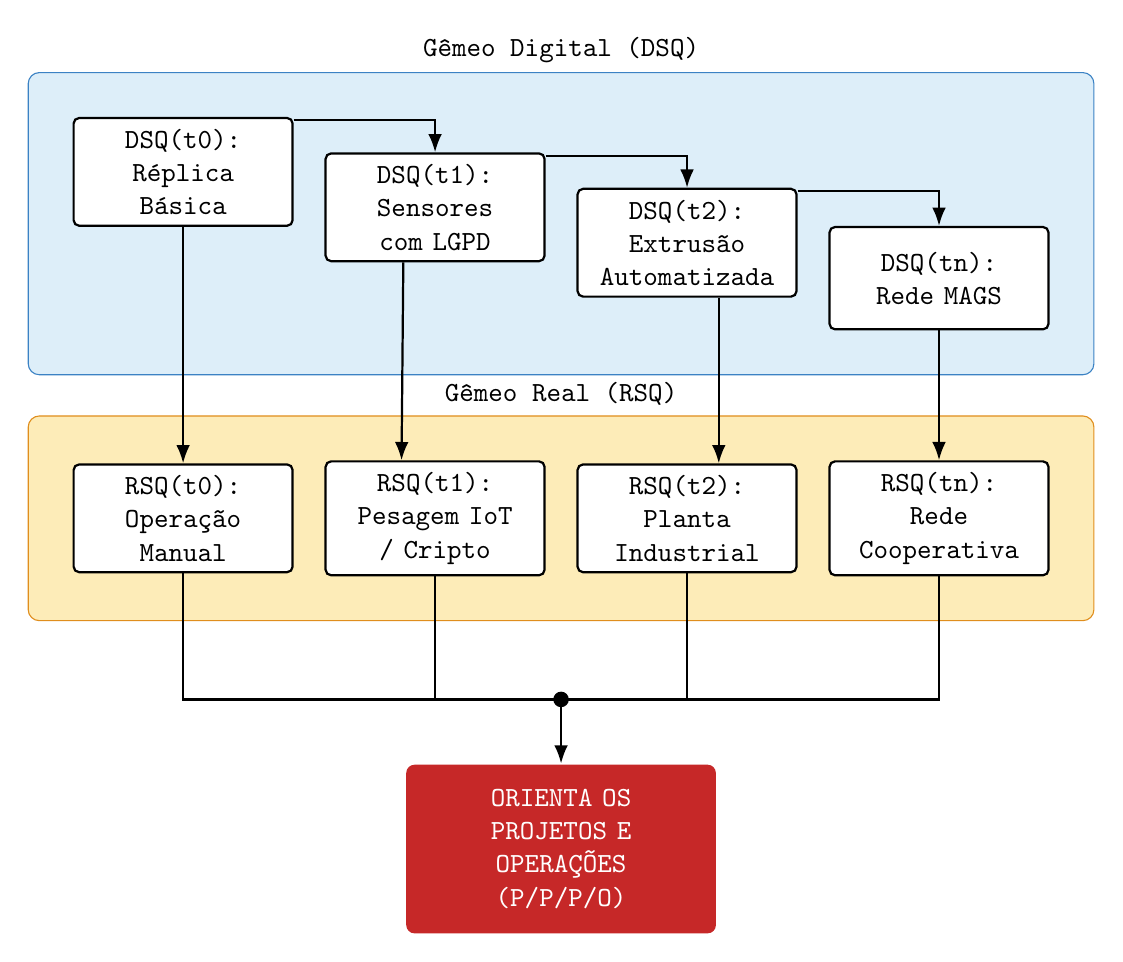
\begin{tikzpicture}[
  font=\ttfamily,
  box/.style={rectangle, draw=black, fill=white, rounded corners=2pt,
              align=center, text width=2.5cm, minimum height=1.3cm, inner sep=4pt},
  >=Latex, thick
]

  % ---- DSQ: ladder horizontal, leve degrau entre blocos ----
  \node[box] (t0) at (0,7.6)   {DSQ(t0):\\ Réplica Básica};
  \node[box] (t1) at (3.2,7.15){DSQ(t1):\\ Sensores com LGPD};
  \node[box] (t2) at (6.4,6.7) {DSQ(t2):\\ Extrusão Automatizada};
  \node[box] (tn) at (9.6,6.25){DSQ(tn):\\ Rede MAGS};

  \draw[->] (t0.25) -- ++(1.5,0) -| (t1.90);
  \draw[->] (t1.25) -- ++(1.5,0) -| (t2.90);
  \draw[->] (t2.25) -- ++(1.5,0) -| (tn.90);

  % ---- RSQ: linha única, alinhada em x com o DSQ correspondente ----
  \node[box] (r0) at (0,3.2)   {RSQ(t0):\\ Operação Manual};
  \node[box] (r1) at (3.2,3.2) {RSQ(t1):\\ Pesagem IoT / Cripto};
  \node[box] (r2) at (6.4,3.2) {RSQ(t2):\\ Planta Industrial};
  \node[box] (rn) at (9.6,3.2) {RSQ(tn):\\ Rede Cooperativa};

  \draw[->] (t0) -- (r0);
  \draw[->] (t1.240) -- (r1.120);
  \draw[->] (t2.300) -- (r2.60);
  \draw[->] (tn) -- (rn);

  % ---- faixas de fundo ----
  \begin{scope}[on background layer]
    \node[fill=blueband, draw=blueborder, rounded corners=4pt,
          fit=(t0)(t1)(t2)(tn), inner sep=16pt,
          label={[font=\ttfamily]above:Gêmeo Digital (DSQ)}] {};
    \node[fill=yellowband, draw=yellowborder, rounded corners=4pt,
          fit=(r0)(r1)(r2)(rn), inner sep=16pt,
          label={[font=\ttfamily]above:Gêmeo Real (RSQ)}] {};
  \end{scope}

  % ---- convergência: nó pequeno (sem caixa esquisita) ----
  \coordinate (conv) at (4.8,0.9);
  \draw (r0) |- (conv); 
  \draw (r1) |- (conv);
  \draw (r2) |- (conv);
  \draw (rn) |- (conv);
  \filldraw[black] (conv) circle (2.4pt);

  % ---- OPÇÃO A: conclusão abaixo, no mesmo eixo vertical ----
  \node[fill=redbox, text=white, font=\ttfamily\bfseries, align=center,
        rounded corners=3pt, text width=3.3cm, inner sep=9pt]
    (concl) at (4.8,-1.0)
    {ORIENTA OS PROJETOS E OPERAÇÕES (P/P/P/O)};
  \draw[->] (conv) -- (concl);

\end{tikzpicture}
\end{document}